


\section{Section 2: Energy Sensors}


In this section is covered the theory behind energy sensors as well as the technologies used. In subsection \ref{subs:321} is started the presentation of the electric energy. Further on, in subsection \ref{subs:322} is covered the energy transducers and in subsection \ref{subs:323} is presented the challenges and requirements of high power measurement in RTS. This section is concluded with the presentation of the technologies used in RTS for energy measurement purposes.

\subsection{Electric Energy Overview}
\label{subs:321}
Energy in form of electricity is the major traction player on the RTS. 
Complementary to the Diesel, this form of energy is distributed along with the rails in catenaries.
As presented in previous section, there are two major ways of rail electrification: AC or DC.

When a train is connected to a DC transmission line, it is possible to exchange energy from and to the catenary, complying to the Kirchhoff's circuit laws. The catenary is considered as a node that has multiple bi-directional power flow elements, specifically, trains and traction substations.

On AC transmission lines, the power flow is directly related to the relation between the voltage and current waveforms, as presented in figures \ref{fig:traction} and \ref{fig:generation}.

\begin{figure}[h!]
	\centering
	\begin{minipage}{.48\textwidth}
		\centering
		%		\vspace{2.5em}
			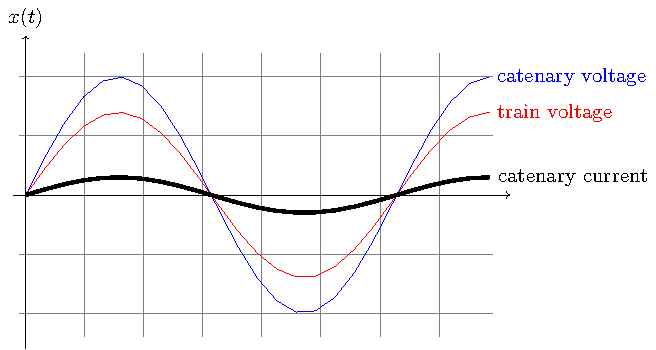
\includegraphics[width=1\textwidth,keepaspectratio]{figures/32.EnergyS/traction}
		%		\vspace{2em}
		\captionof{figure}{Waveforms in traction mode.}
		\label{fig:traction}
	\end{minipage}%
	\begin{minipage}{.01\textwidth}  ~\end{minipage}	
	\begin{minipage}{.48\textwidth}
		\centering
		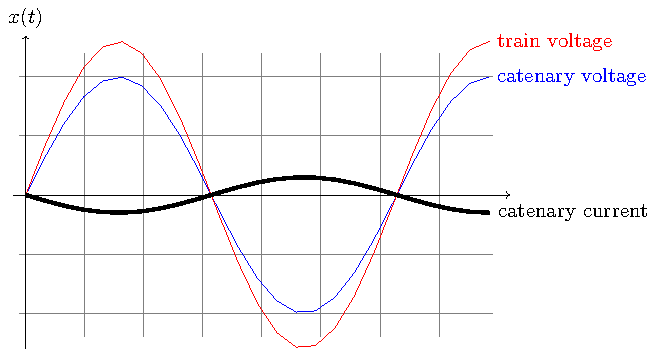
\includegraphics[width=1\textwidth,keepaspectratio]{figures/32.EnergyS/generation}

		
		%		\vspace{0.5em}
		\captionof{figure}{Waveforms in generation mode.}
		\label{fig:generation}
	\end{minipage}
\end{figure}

The energy calculation depends on the voltage and currents measured in the catenary. This function present in train energy meters evaluates the voltage and currents and generates the active, reactive and power factor information of the train. In figure \ref{fig:liran2014} is presented an example of the energy information 1h operation of {$HX_D1B$} locomotive.


\begin{figure}[h!]
	\centering
	\begin{minipage}{0.8\textwidth}
		\centering
				\vspace{-0.75em}
		\includegraphics[width=0.75\textwidth,keepaspectratio]{figures/32.EnergyS/liran2014}
				\vspace{-0.75em}
		\captionof{figure}{1h waveforms of active power (black), reactive power (red) and power factor (blue) of {$HX_D1B$} locomotive.  Adapted from \cite{liran2014}.}
		\label{fig:liran2014}
	\end{minipage}%
	
\end{figure}


\subsection{Current transducers and voltage transducers}
\label{subs:322}	
	According to \cite{webster2012}, a transducer is a device capable to convert different physical signal forms. In the scope of energy measurements, current and voltage transducers are employed. These devices converts the field energy waveforms into a voltage (or current) waveform capable of be acquired by a processing unit (such as a microcontroller, PLC, etc).
	
	
a.	Commonly used technologies and principles
b.	New breakthroughs

\subsection{High power measurement challenges in RTS}	
\label{subs:323}


\subsection{Energy measurement technologies in RTS }
\label{subs:324}

